\documentclass{standalone}
  \usepackage{tikz}
  \usetikzlibrary{arrows, automata, positioning}
  \tikzstyle{automaton}=[shorten >=1pt, node distance=2cm, pos=.4,
                         >=stealth', initial text=]
  \tikzstyle{accepting}=[accepting by arrow]

\begin{document}
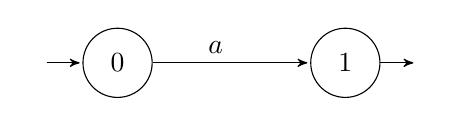
\begin{tikzpicture}[automaton]
  \node[state,initial] (0) {$0$};
  \node[state,accepting] (1) [right=of 0] {$1$};
  \path[->] (0) edge node[above] {$a$} (1);
\end{tikzpicture}
\end{document}
